%template for simulation report

\newpage

\section{Super Nova Remnant G1.9+0.3}

\textbf{Object Description:} G1.9+0.3: It's less than 2' across

\textbf{Simulation Period:} March 2011
% month and year

\textbf{Science Team contract:} Stephen Reynolds

\textbf{NuSIM configuration file:}

\textbf{Exposure time:} 200 ks

\textbf{Input Source:} Chandra image with 0.492" pixels.  Spectrum is F = 7.e-6 (E/10 keV)$^{-1}$ exp(-sqrt(E/2.2 keV)) ph cm$^{-2}$ s$^{-1}$ keV$^{-1}$ 

\textbf{Tiling Method:} Spherical pointing pattern of 9 

\textbf{OA Database Version:} 007
% fill in version number e.g. 008

\textbf{Mast Bend Database:} SAA 135
% fill in SAA number

\textbf{Simulation notes:} 
% did we learn anything, did we have to do something special?

\textbf{Status:} 
% are more simulations pending? is it missing something? 

\textbf{Location and name of simulation output:} resource/examples/G1.9 in the nusim SVN distribution

\begin{figure}[h]
\begin{center}
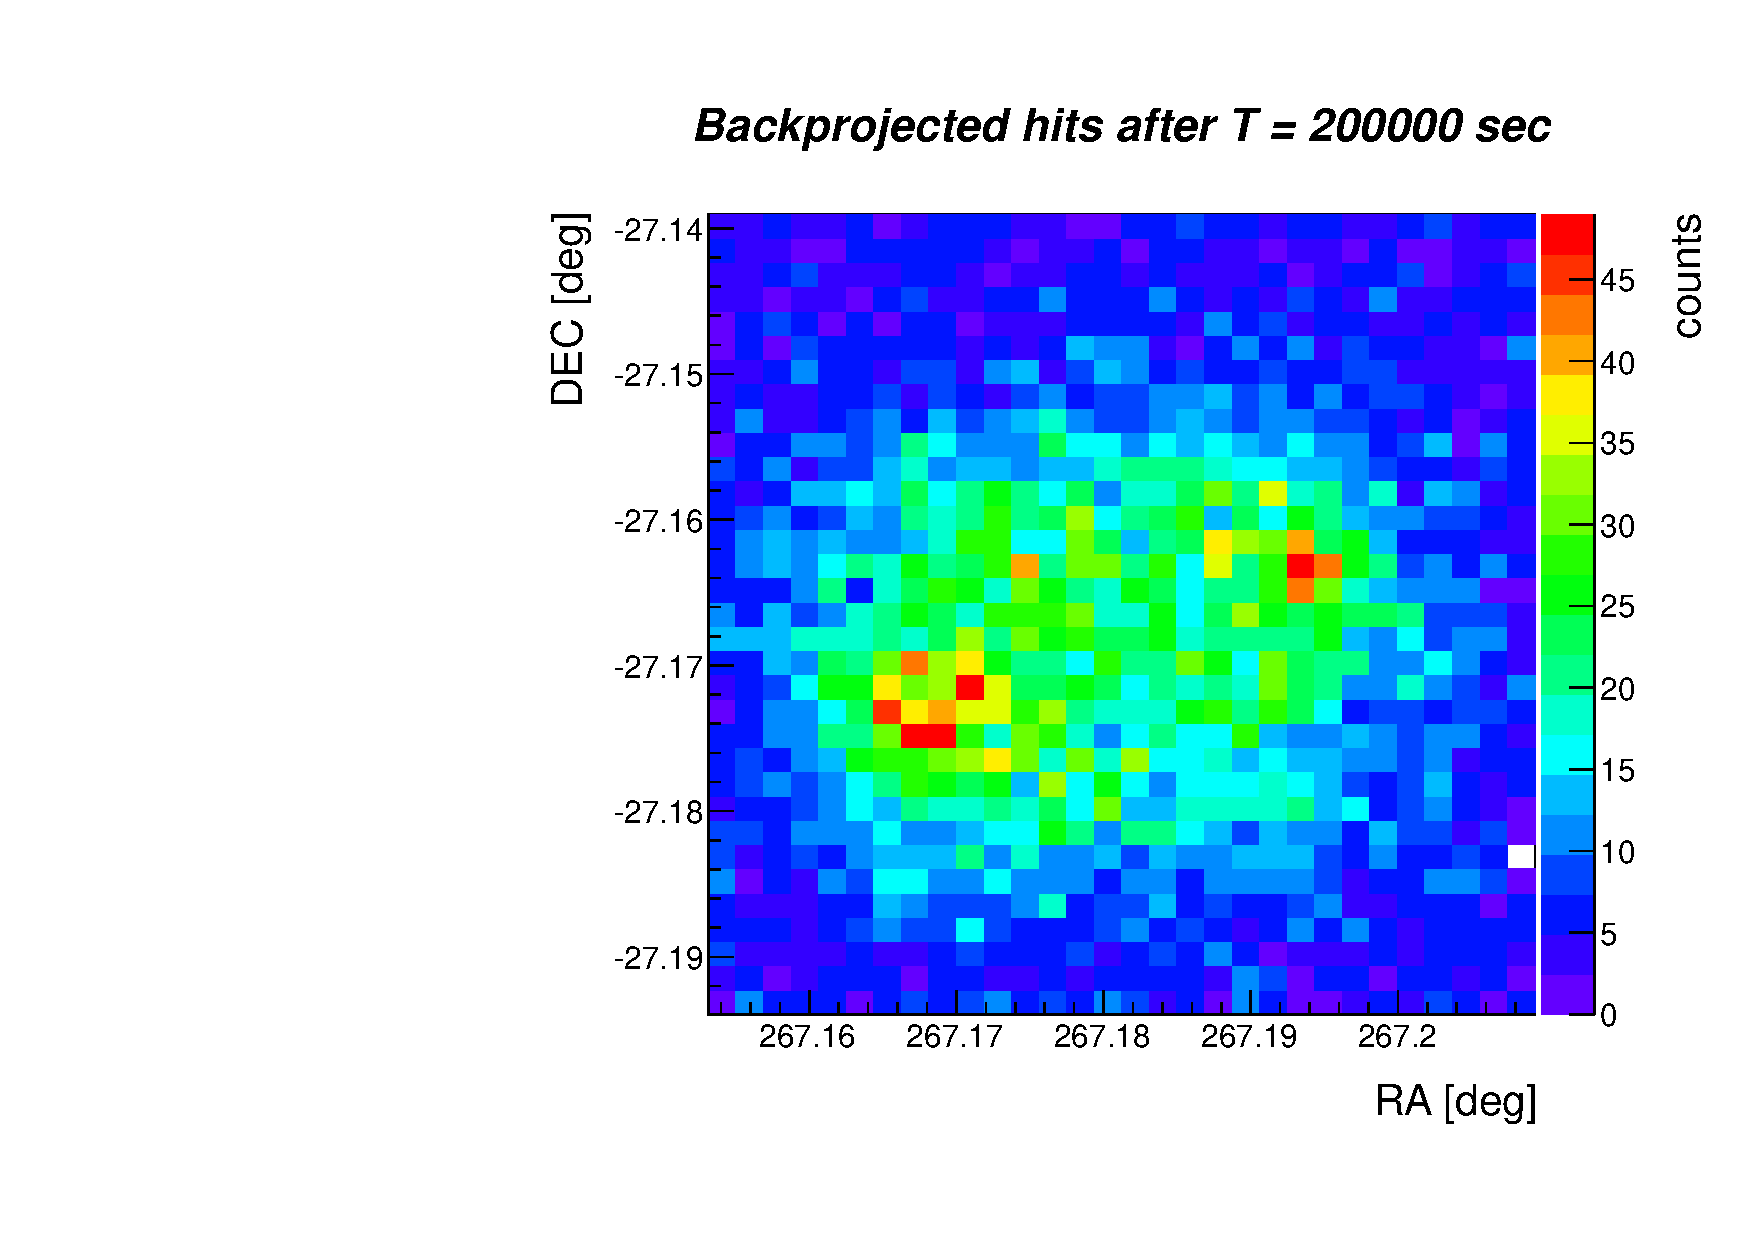
\includegraphics[width=10cm]{G1.9/G19.pdf}  % if there is an image put it here  
\caption{G1.9+0.3.}
\label{g19} 
\end{center}
\end{figure}

